\documentclass[10 pt]{article}

\usepackage[utf8x]{inputenc}
\usepackage{dsfont}
\usepackage{amsthm}
\usepackage{amsfonts}
\usepackage{tensor}
\usepackage{mathtools}
\usepackage[T1]{fontenc}
%\usepackage[spanish]{babel}
\usepackage[cm]{fullpage}
\usepackage{graphicx}
\usepackage{float}
\usepackage{bm}
\usepackage{setspace}
\usepackage{enumitem}
\usepackage{mdwlist}
\usepackage{parskip}
\usepackage{listings}
\usepackage{color}
%\usepackage{epstopdf}
\usepackage{tikz,datatool}
\usepackage{hyperref}

\newcommand{\HRule}{\rule{\linewidth}{0.5mm}}

\AtBeginDocument{
  \let\myThePage\thepage
  \renewcommand{\thepage}{\oldstylenums{\myThePage}}
}

\newcommand{\gra}{$^\text{o}$}
\newcommand{\dif}{\text{d}}
\newcommand{\avg}[1]{\left\langle #1 \right\rangle}
\newcommand{\ket}[1]{\left| #1 \right\rangle}
\newcommand{\bra}[1]{\left\langle #1 \right|}
\newcommand{\bket}[2]{\left\langle #1 \middle| #2 \right\rangle}
\newcommand{\der}[2]{\frac{\text{d} #1}{\text{d} #2}}
\newcommand{\prt}[2]{\frac{\partial #1}{\partial #2}}
\newcommand{\dert}[3]{\frac{\text{d}^#3 #1}{\text{d} #2^#3}}
\newcommand{\prtt}[3]{\frac{\partial^#3 #1}{\partial #2^#3}}
\newcommand{\dl}{\mathcal{L}}
\newcommand{\dha}{\mathcal{H}}
\newcommand{\vol}{\text{vol}}
\renewcommand{\vec}[1]{\pmb{#1}}

\newenvironment{algo}[1]
{  \begin{center}
   \mbox{
       \begin{minipage}{\textwidth}
           \begin{tabbing}
           \settabs
            #1
           \end{tabbing}
        \end{minipage}
    }
    \end{center}
}{}
\newcommand{\settabs}{mmm\=mmm\=mmm\=mmm\=mmm\=mmm\=\kill}

\DeclarePairedDelimiter\ceil{\lceil}{\rceil}
\DeclarePairedDelimiter\floor{\lfloor}{\rfloor}

\definecolor{mygray}{rgb}{0.4,0.4,0.4}
\definecolor{mygreen}{rgb}{0,0.5,0.25}
\definecolor{myorange}{rgb}{1.0,0.4,0}

\definecolor{clock0}{cmyk}{1,0,0,0}
\definecolor{clock1}{cmyk}{1,1,0,0}
\definecolor{clock2}{cmyk}{0,1,0,0}
\definecolor{clock3}{cmyk}{0,1,1,0}
\definecolor{clock4}{cmyk}{1,0,1,0}
\definecolor{clock5}{cmyk}{1,1,1,0}
\definecolor{clock6}{cmyk}{0,0,1,0}
\definecolor{clock7}{cmyk}{0,0,0,0.1}

\begin{document}

\lstset{
language=C++,
basicstyle=\ttfamily\color{black},
commentstyle=\color{mygray}\ttfamily,
frame=single,
numbers=left,
numbersep=5pt,
numberstyle=\tiny\color{mygray}\ttfamily,
keywordstyle=\color{mygreen}\ttfamily,
showspaces=false,
showstringspaces=false,
stringstyle=\color{myorange}\ttfamily,
tabsize=2,
emph={double,uint8_t,uint16_t,uint32_t,uint64_t,int8_t,int16_t,int32_t,int64_t},
emphstyle={\color{blue}\ttfamily}
}

\begin{center}
  \Large \textsc{Week 5: Pair correlation function using MC simulations in the NVT ensemble}
\end{center}

\begin{center}
  \large \textsc{Francisco García Flórez}
\end{center}

<<<<<<< HEAD
\section{Pair correlation function}

The way we defined this pair correlation function, $g(r)$, will count some number of particles depending on $r$, that will converge to the density of the system when considering the limit $r \rightarrow \infty$. Although, because of the normalization factor $1/\rho$ in front, in this limit it will then go to one.

\section{Results}

Simulating a system in the NVT ensemble with the initial configuration of a FCC lattice with different distances between spheres, and then computing the distance probability density gives us the following results:

\begin{figure}[H]
  \begin{center}
    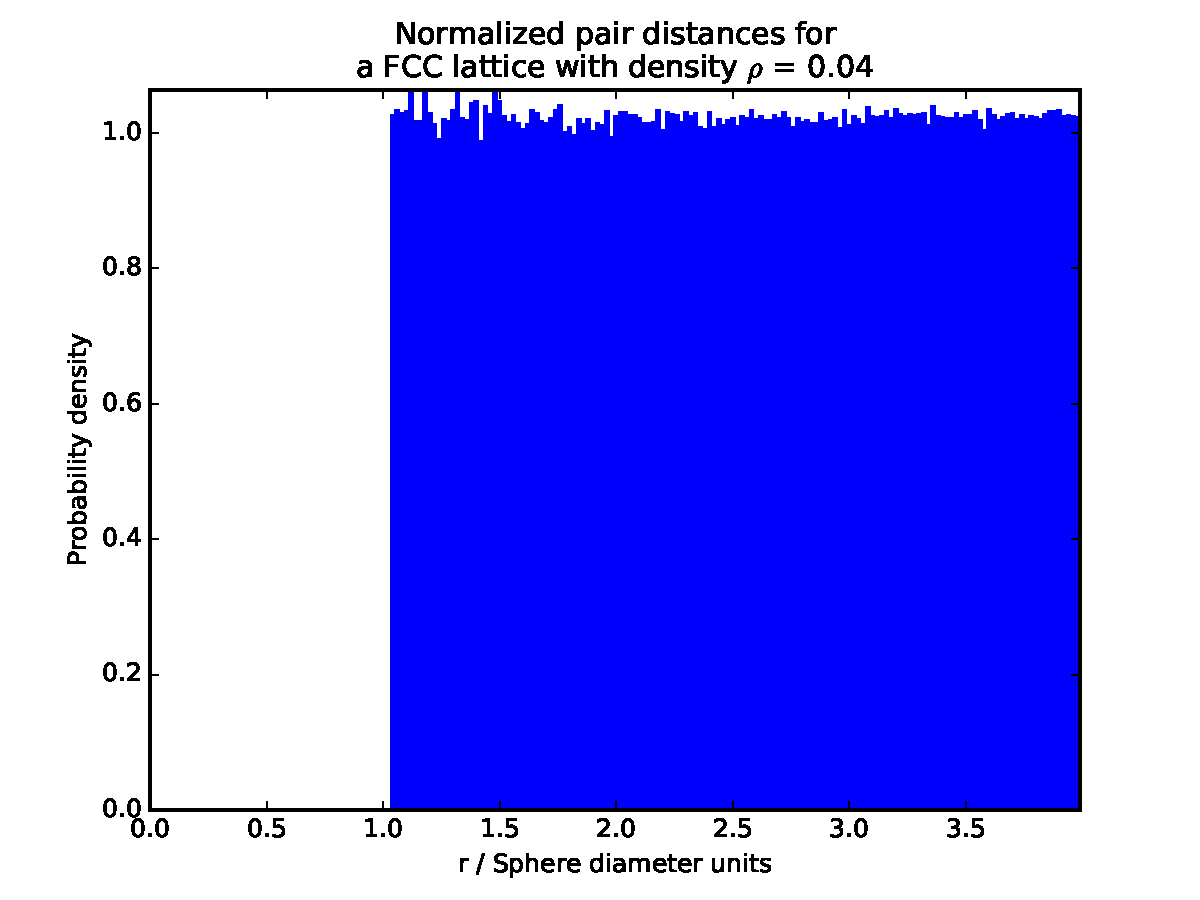
\includegraphics[width=0.49\textwidth]{{../graphs/fcc-0.04}.pdf}
    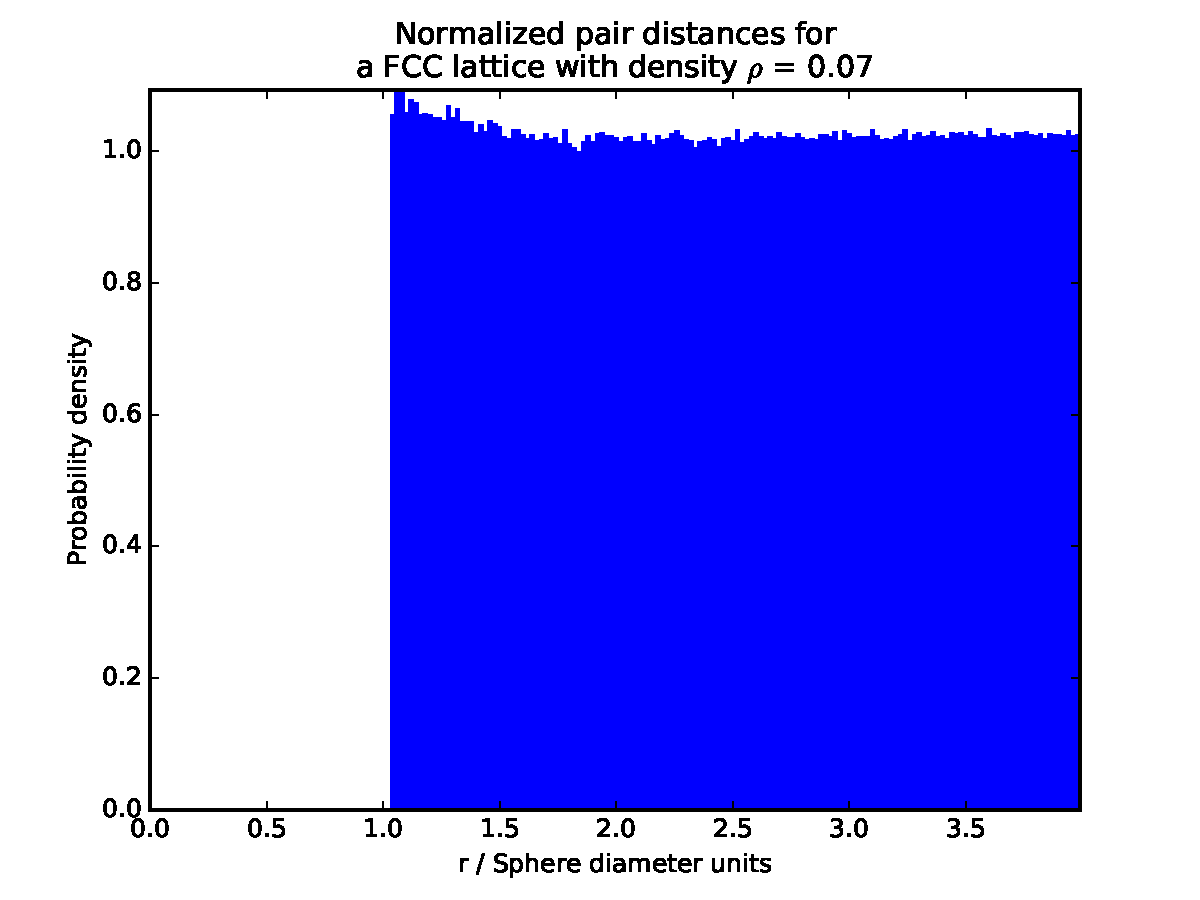
\includegraphics[width=0.49\textwidth]{{../graphs/fcc-0.07}.pdf}
  \end{center}
\end{figure}

\begin{figure}[H]
  \begin{center}
    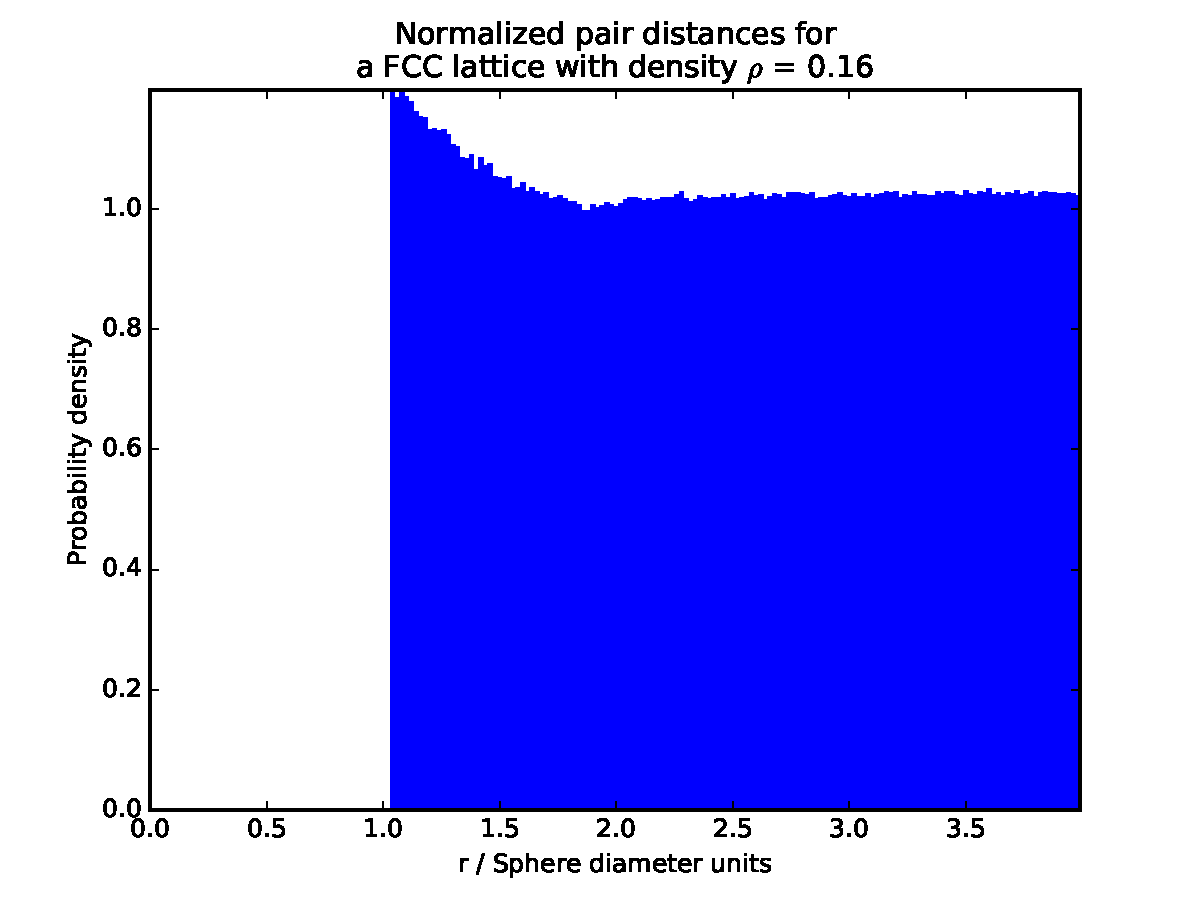
\includegraphics[width=0.49\textwidth]{{../graphs/fcc-0.16}.pdf}
    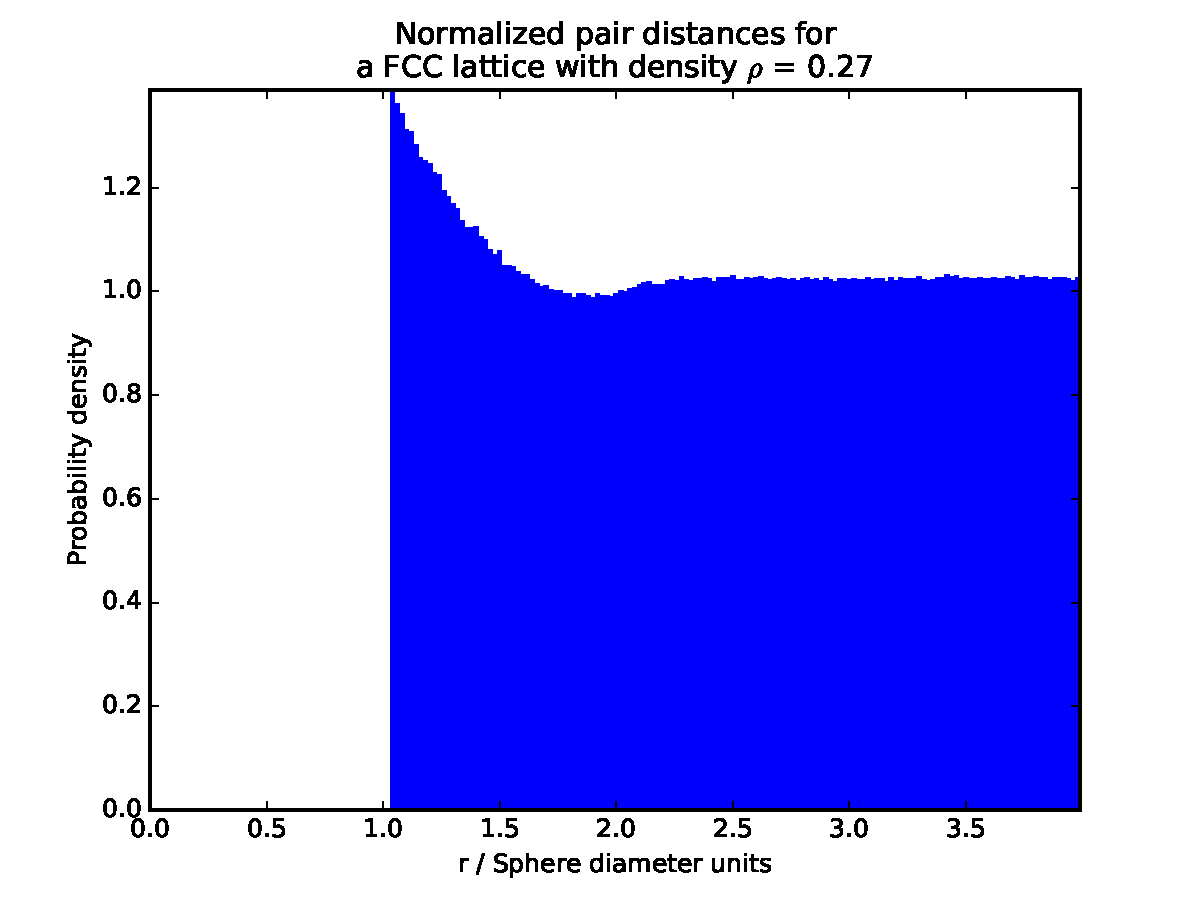
\includegraphics[width=0.49\textwidth]{{../graphs/fcc-0.27}.pdf}
  \end{center}
\end{figure}

\begin{figure}[H]
  \begin{center}
    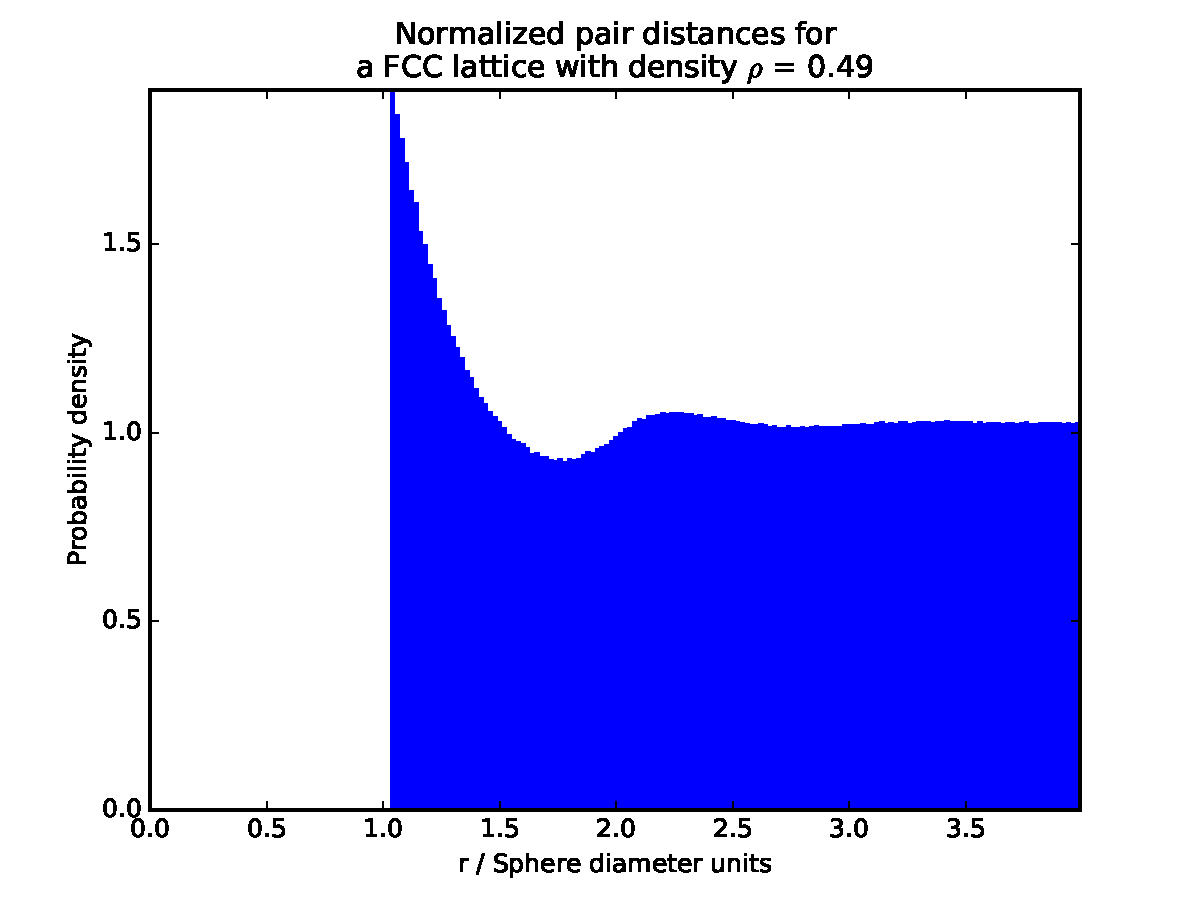
\includegraphics[width=0.49\textwidth]{{../graphs/fcc-0.49}.pdf}
    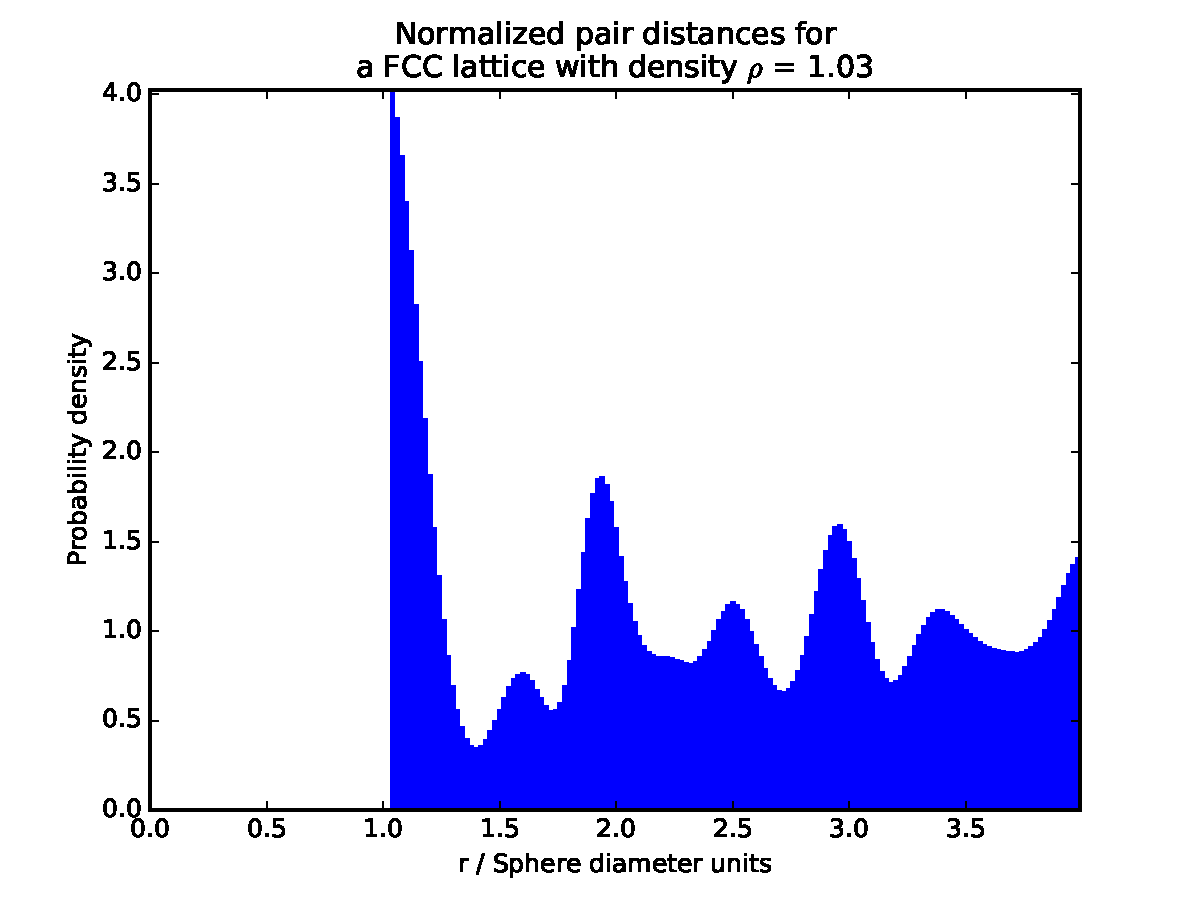
\includegraphics[width=0.49\textwidth]{{../graphs/fcc-1.03}.pdf}
  \end{center}
\end{figure}

As we were expecting, it goes to one as $r$ increases. Now, notice that for $\rho \ll 1$ we find a result really close to an ideal gas, as particles interact less. When the density increases some patterns become significant, reflecting the layered configuration of the fluid phase. In the extreme case of a solid, we can perfectly see peaks and valleys at the right distances for a FCC lattice.

In this latter case, we can specifically notice how we can find several sets of peaks, each one corresponding to different layers that we can find in the lattice seen from one specific location. If we were doing more simulations for $\rho \in [0.5, 1.0]$ we would be seeing this transition from a slight valley with small oscillations to the lattice pattern.
=======

>>>>>>> 8ebc1ce7c21bb664fa948fa5f207337baaed4f64

\end{document}
